Suppose that feedback system has a delay of $T_{d}$ seconds in reporting sensor data so that the feedback system is
\begin{center}
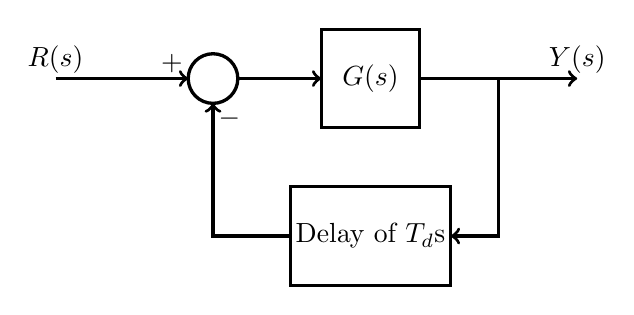
\begin{tikzpicture}[scale=1,inner sep=0pt,outer sep=0pt,very thick,
sysblock/.style={draw,rectangle,inner sep=2pt,minimum width=1.25cm,minimum height=1.25cm,very thick}]
\draw (2,0) node[draw,circle] (sum1) {$\rule{0pt}{18pt}$};
\draw (4,0) node[sysblock] (G) {$G(s)$};
\draw (4,-2) node[sysblock] (D) {Delay of $T_{d}$s};
\draw[->] (0,0) node[above=2pt] {$R(s)$} -- (sum1.180) node[above left=2pt] {$+$};
\draw[->] (sum1.0) --  (G);
\draw[->] (G.0) -- ++(2,0) node[above=2pt] {$Y(s)$};
\draw[->] (G.0) ++(1,0) |- (D.0);
\draw[->] (D.180)  -| (sum1.-90) node[below right=2pt] {$-$};
\end{tikzpicture}
\end{center}
The frequency response of $G(s)$ is shown below. 
\begin{center}
\includegraphics[width=5in]{\mainfolder/LectureNotes/\lecturefolder/HomeworkProblems/Problem01/bode2.pdf}
\end{center}
\begin{enumerate}[(a)]
\item If $T_{d}=0$, find the phase and gain margins. 
\item What is the maximum value for $T_{d}$ that can be tolerated before the closed loop system becomes unstable?
\end{enumerate}
